\chapter{Related work} % Main chapter title

\label{Chapter2} % Change X to a consecutive number; for referencing this chapter elsewhere, use \ref{ChapterX}


%----------------------------------------------------------------------------------------
%	SECTION 1
%----------------------------------------------------------------------------------------
\section{Redirected walking}%\cite{7892373}
In a virtual environment, there are many variations in size, so it is difficult to bring a physical space that is consistent with the virtual environment.



Redirected Walking~\cite{7892373} is a VR locomotion technique. A user is redirected by applying several gains to a virtual camera that generates screen imagery displayed in an HMD the user wears. There are 4 types of gains: a translation gain, a curvature gain, a rotational gain, and a time dependent rotational gain~\cite{10.2312:egs.20011036}\cite{10.1145/1450579.1450611}. This method can provide the user with a path to walk around the virtual environment without colliding with walls in the physical space.

\subsubsection{Translation gains}
If a virtual environment has a walking path that is farther than the physical space, it is difficult for users to explore the virtual environment. 

A translation gain (Fig.~\ref{fig:TGain}) controls walking distance of a user in the physical space. The walking speed of the user in the virtual environment is obtained by multiplying the translation gain and the walking speed in the physical space together. 
\[
Translation\;gain =\frac{ Virtual\;walking\;distance}{ Real\;walking\;distance}
 \]

\begin{figure}[H]\centering
	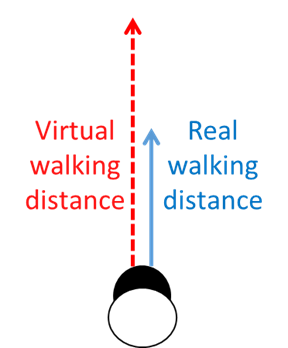
\includegraphics[width=0.27\textwidth]{Pictures/TranslationGain.png}%imagine location
	\caption{Translation gain.}\label{fig:TGain}%use name for ref.
\end{figure}


%%%%%%%%%%%%%%%%%%%%%%%%%%%%%%%
\subsubsection{Curvature gains}
When an obstacle is found in front of a user in the physical space while the user is walking, creating an illusion of having the user walk in curve to dodge the obstacle.

A curvature gain (Fig.~\ref{fig:CGain}) redirects a walking path of the user in the physical space. The coordinates of the virtual environment are rotated while the user is walking so that his/her walking path in the physical space is curved. 
\[
Curvature\;gain =\frac{ Radius\;of\;the\;curvature\;in\;the\;virtual\;world}{Radius\;of\;the\;curvature\;in\;the\;real\;world}
 \]
\begin{figure}[H]\centering
	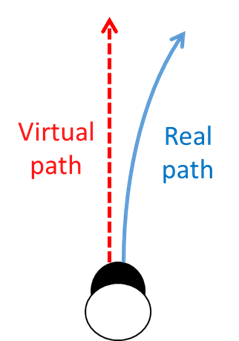
\includegraphics[width=0.25\textwidth]{Pictures/CurvatureGain.png}%imagine location
	\caption{Curvature gain.}\label{fig:CGain}%use name for ref.
\end{figure}

%%%%%%%%%%%%%%%%%%%%%%%%%%%%%%%%%%%
\subsubsection{Rotational gains}
When a user wears an HMD, his/her position and direction are tracked via a postural position of the HMD, and they could be used to avoid areas that might cause collisions with obstacles. Reorientation of the user to face a wider area or no other obstacles to reduce the chance of collisions, is an option.

A rotational gain (Fig.~\ref{fig:RGain}) reorients the facing direction of a user in the physical space. The turning speed of the user in the virtual environment is obtained by multiplying the rotational gain and the turning speed in the physical space together.
\[
Rotation\;gain =\frac{Virtual\;rotation}{Real\;rotation}
 \]
\begin{figure}[H]\centering
	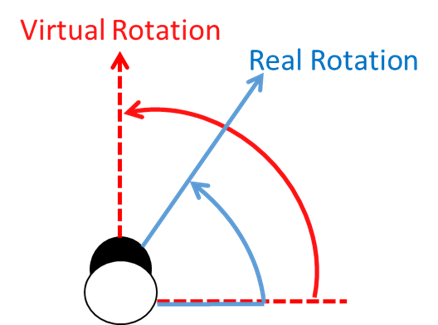
\includegraphics[width=0.4\textwidth]{Pictures/RotationGain.png}%imagine location
	\caption{Rotational gain.}\label{fig:RGain}%use name for ref.
\end{figure}
\newpage
%%%%%%%%%%%%%%%%%%%%%%%%%%%%%%%%%%%%%%%%%
\subsubsection{Time-dependent rotational gains}
Collision prediction is an important factor in activating the collision avoidance function. In this method, the degree of rotation depends on the specified time.

Time-dependent rotational gains (Fig.~\ref{fig:T2DGain}) redirects the direction the user is facing in their physical space. The coordinates of the virtual environment are rotated constantly as the time passed so that the direction the user is facing in their physical space is changed.
\[
Time\;dependent\;rotational\;gain = Virtual\;rotation * Time
 \]
\begin{figure}[H]\centering
	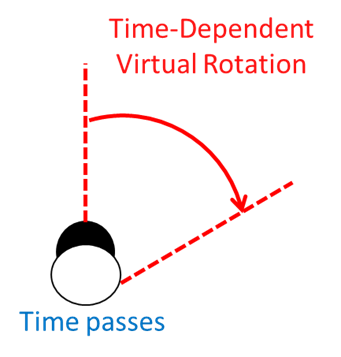
\includegraphics[width=0.35\textwidth]{Pictures/TimeDependentRotationGain.png}%imagine location
	\caption{Time-dependent rotational gain.}\label{fig:T2DGain}%use name for ref.
\end{figure}
\newpage
%%%%%%%%%%%%%%%%%%%%%%%%%%%%%
%\vspace{5mm}
\subsubsection{Steer to Center}
Steer to Center~\cite{6549377} is one of VR locomotion techniques based on Redirected Walking and it helps a user avoid collisions with the physical walls in his/her room. The user is steered toward the center of the room by rotational gains. The rotation direction is depending on the quickest direction to return to the center. The process of S2C is shown in Fig.~\ref{fig:S2C_detect_1}-\ref{fig:S2C_steer_2}.
\begin{figure}[H]\centering
	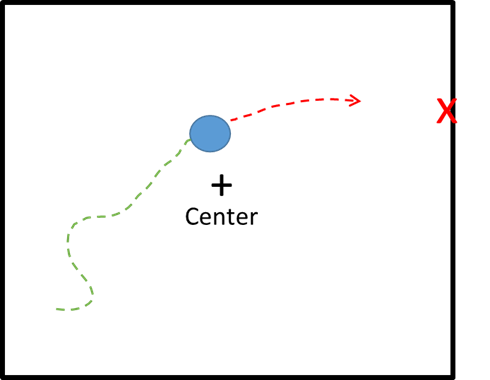
\includegraphics[width=0.6\textwidth]{Pictures/Predict the collision with the wall.png}%imagine location
	\caption{Predict the collision with the wall.}\label{fig:S2C_detect_1}%use name for ref.
\end{figure}
\begin{figure}[H]\centering
	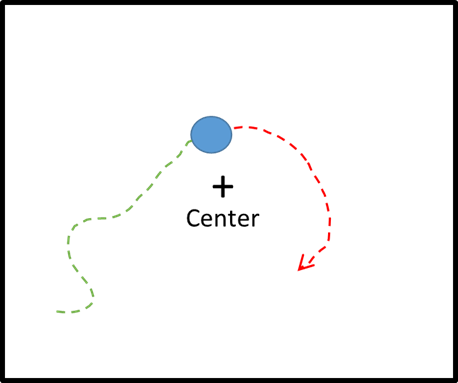
\includegraphics[width=0.6\textwidth]{Pictures/Steer the user to the center.png}%imagine location
	\caption{Steer the user to the center.}\label{fig:S2C_steer_2}%use name for ref.
\end{figure}
\newpage
%%%%%%%%%%%%%%%%%%%%%%%%%%%%%%%%%%%%%%%%%%%
\section{Collision avoidance for two users}
\subsubsection{Steer to Offset Center}
Steer to Offset Center~\cite{6549377} (S2OC) is a collision avoidance method for two users based on the S2C method. S2C is designed for one user in a physical space to deal with collisions with walls. S2OC defines two target points for two users. A collision is predicted and the users are steered to the closest target point to avoid the collision. The distance between the center point and target points, depends on the physical space.
\begin{figure}[H]\centering
	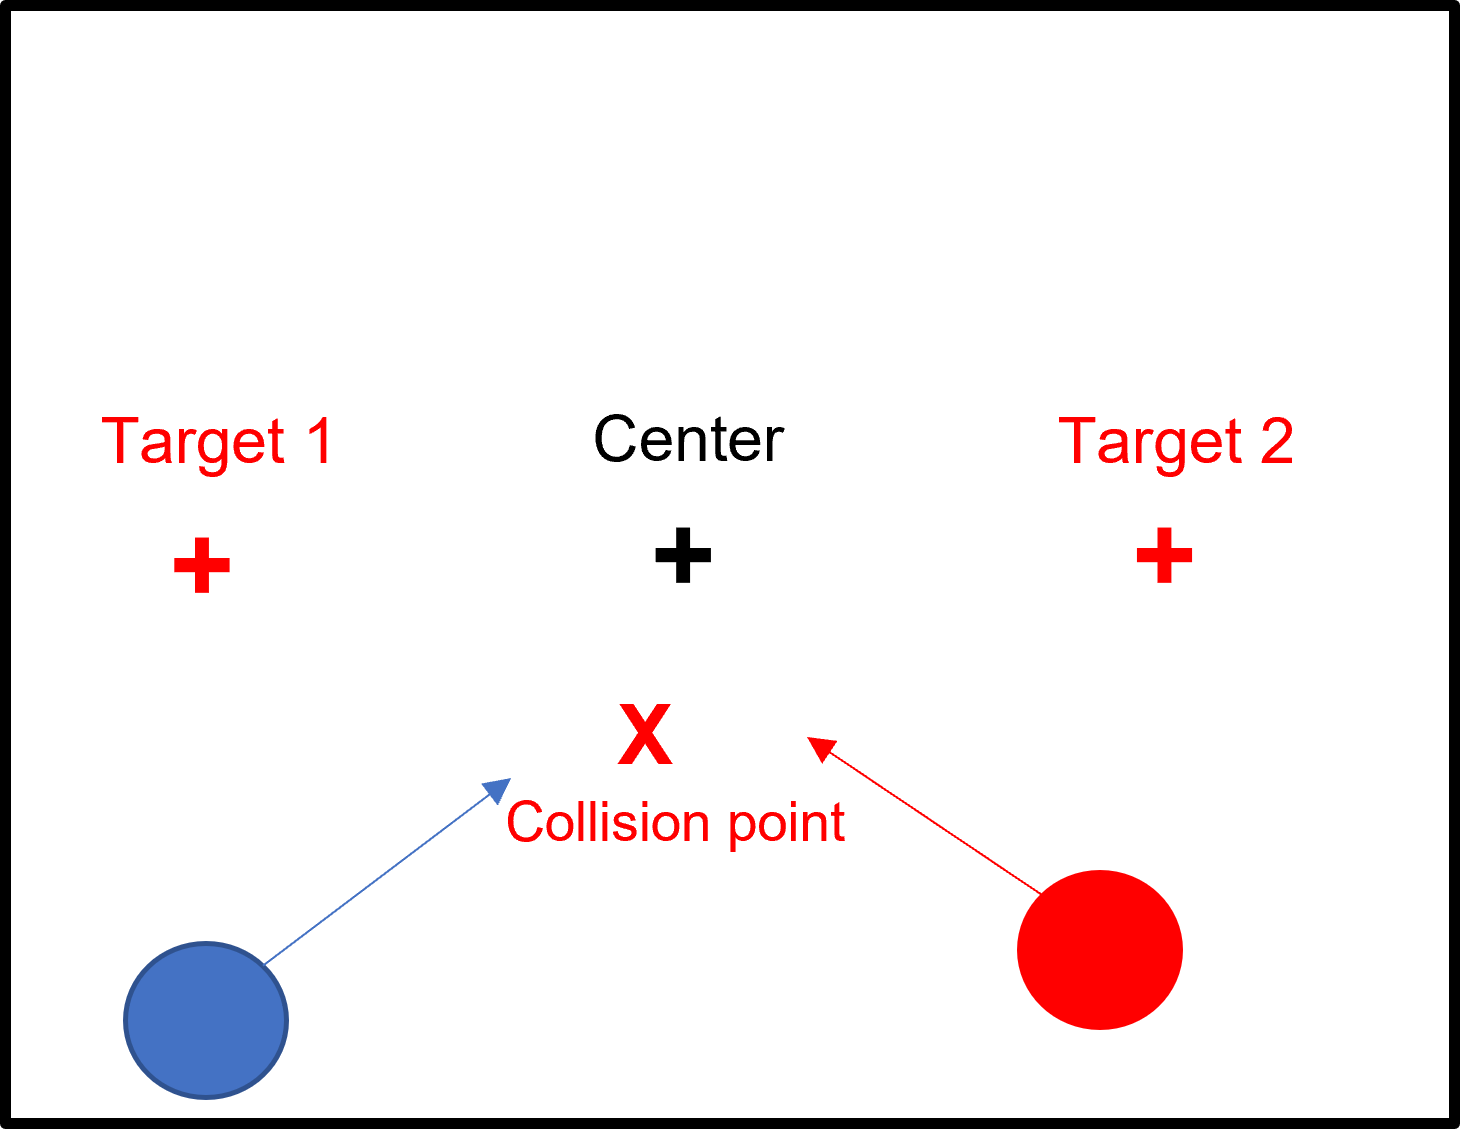
\includegraphics[width=0.65\textwidth]{Pictures/OffsetCenter_1.png}%imagine location
	\caption{Predict a collision.}\label{fig:S2OC_detect_1}%use name for ref.
\end{figure}
\begin{figure}[H]\centering
	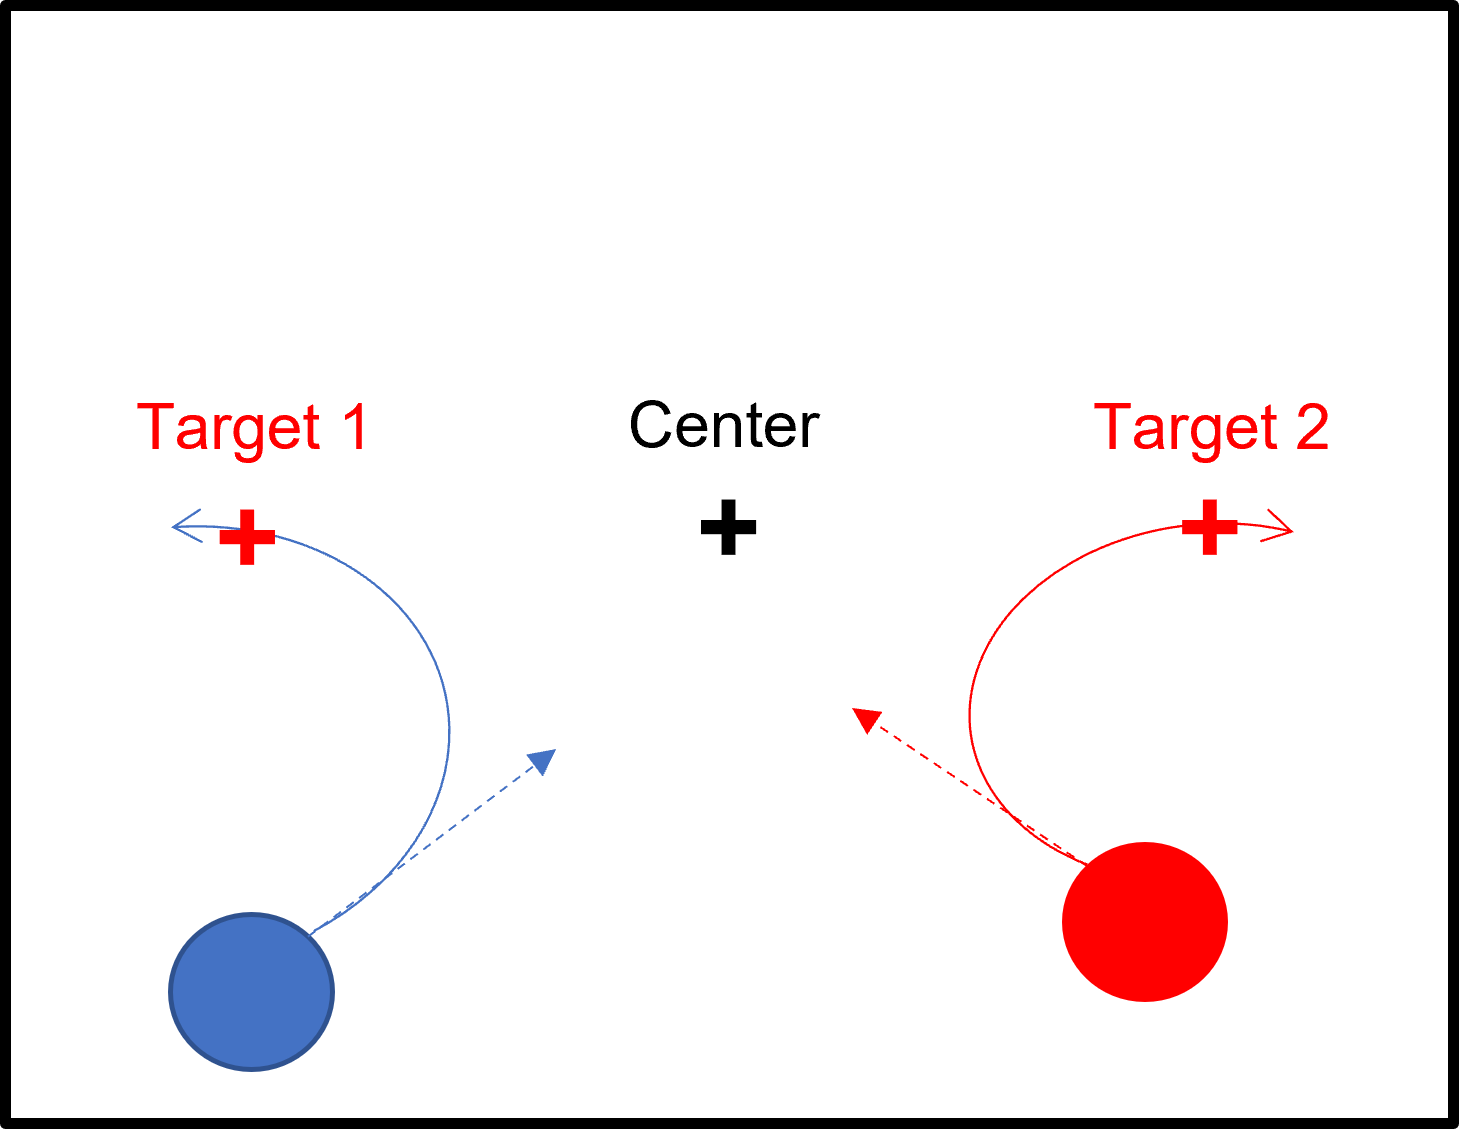
\includegraphics[width=0.65\textwidth]{Pictures/OffsetCenter_2.png}%imagine location
	\caption{Steer the users to the closest target.}\label{fig:S2OC_steer_2}%use name for ref.
\end{figure}
\newpage

\section{Collision avoidance for multiple users}

%%%%%%%%%%%%%%%%%%%%%%%%%%%%%%
J. Holm et al.~\cite{6549377} discusses a collision avoidance method for multiple users, meaning more than two users. Their method consists of four components: position prediction,  walking direction prediction, collision detection and collision avoidance.

T. Dong et al.~\cite{8798319} applies the Holm's method to physical space management for multiple users. The physical space management divides a physical space into subspaces by clustering around the users. The maximum number of users in each subspace is three.


%%%%%%%%%%%%%%%%%%%%%%%%%%%%%%

\subsubsection{Position prediction}
 To predict a collision, positions and walking directions of users are significant. The next positions of users are predicted by calculating their walking directions and the previous positions.
\subsubsection{Walking direction prediction}

A walking direction is predicted by linear regression from a sequence of the previous positions to determine the slope (Fig.~\ref{fig:Walking prediction}).


%First, record the user walking into the sequence of the previous positions. The user's direction (slope of the predicted line) is predicted by linear regression from a sequence of the previous positions. Linear regression is employed to deliver predictions about the value of one variable based on the value of another. The predicted distance depends on the distance of the previous positions and the sequence of the previous positions is recorded upon the setting time. After getting the slope and distance, the user's position in the future is predicted from these data. %The walking prediction shown in Fig.~\ref{fig:Walking prediction.



\begin{figure}[H]\centering
	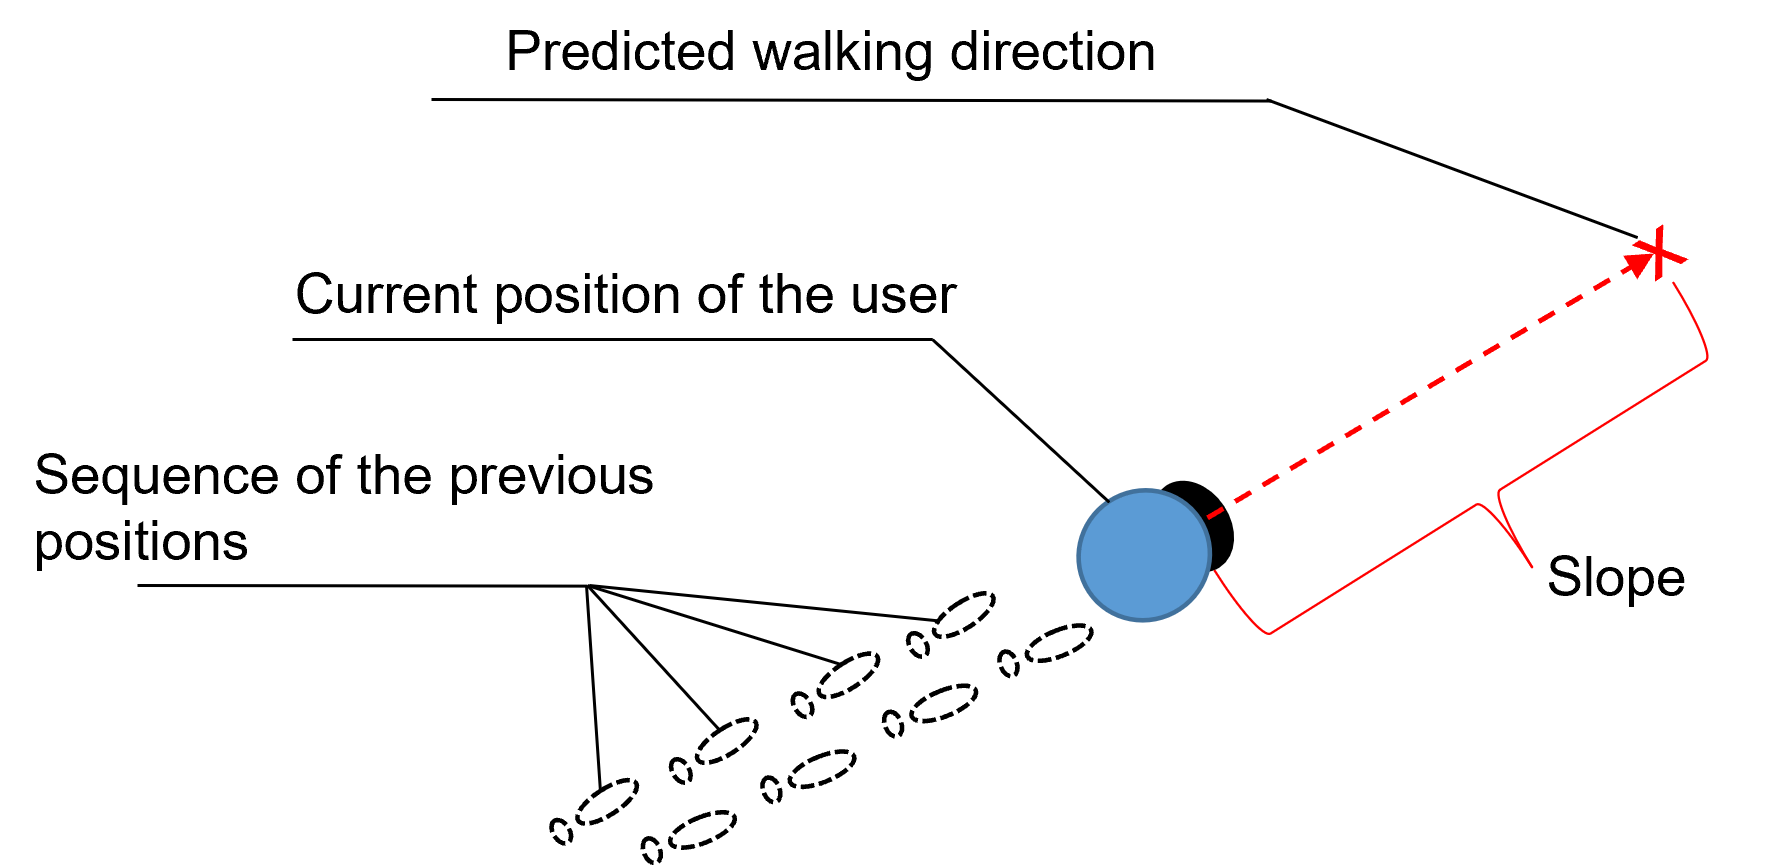
\includegraphics[width=1.0\textwidth]{Pictures/Walking prediction.png}%imagine location
	\caption{Walking prediction.}\label{fig:Walking prediction}%use name for ref.
	
\end{figure}




%Straight line formula:
%\[
 %y = xm + c
 %\]
%\[
%m = \frac{\upDelta y}{\upDelta x}
%\]
%\[
%c = y - xm
% \]

%\[
%Distance = \sqrt{\upDelta x^2 + \upDelta y^2}
 %\]
%\\

%\hspace{10mm}$\upDelta x$  = The changing value in the horizontal axis.

%\hspace{10mm}$\upDelta y$ = The changing value in the vertical axis.

%\hspace{10mm} c = Constant value of equation.

%\hspace{10mm} m = Slope of a straight line.

%\hspace{10mm} Distance = Distance between current position and next position on straight line.
%\\


\newpage
\subsubsection{Collision detection}
Predicting sequences of next positions of users, the next step is to detect a collision point. The collision detection uses circular equations to detect the collision point, shown in Fig.~\ref{fig:Collision detection}.

The collision point is obtained by substituting positions of users into circular equations and using the equalization of those equations to find the intersection.

The circle radius is the average width of a human shoulder.



\begin{figure}[H]\centering
	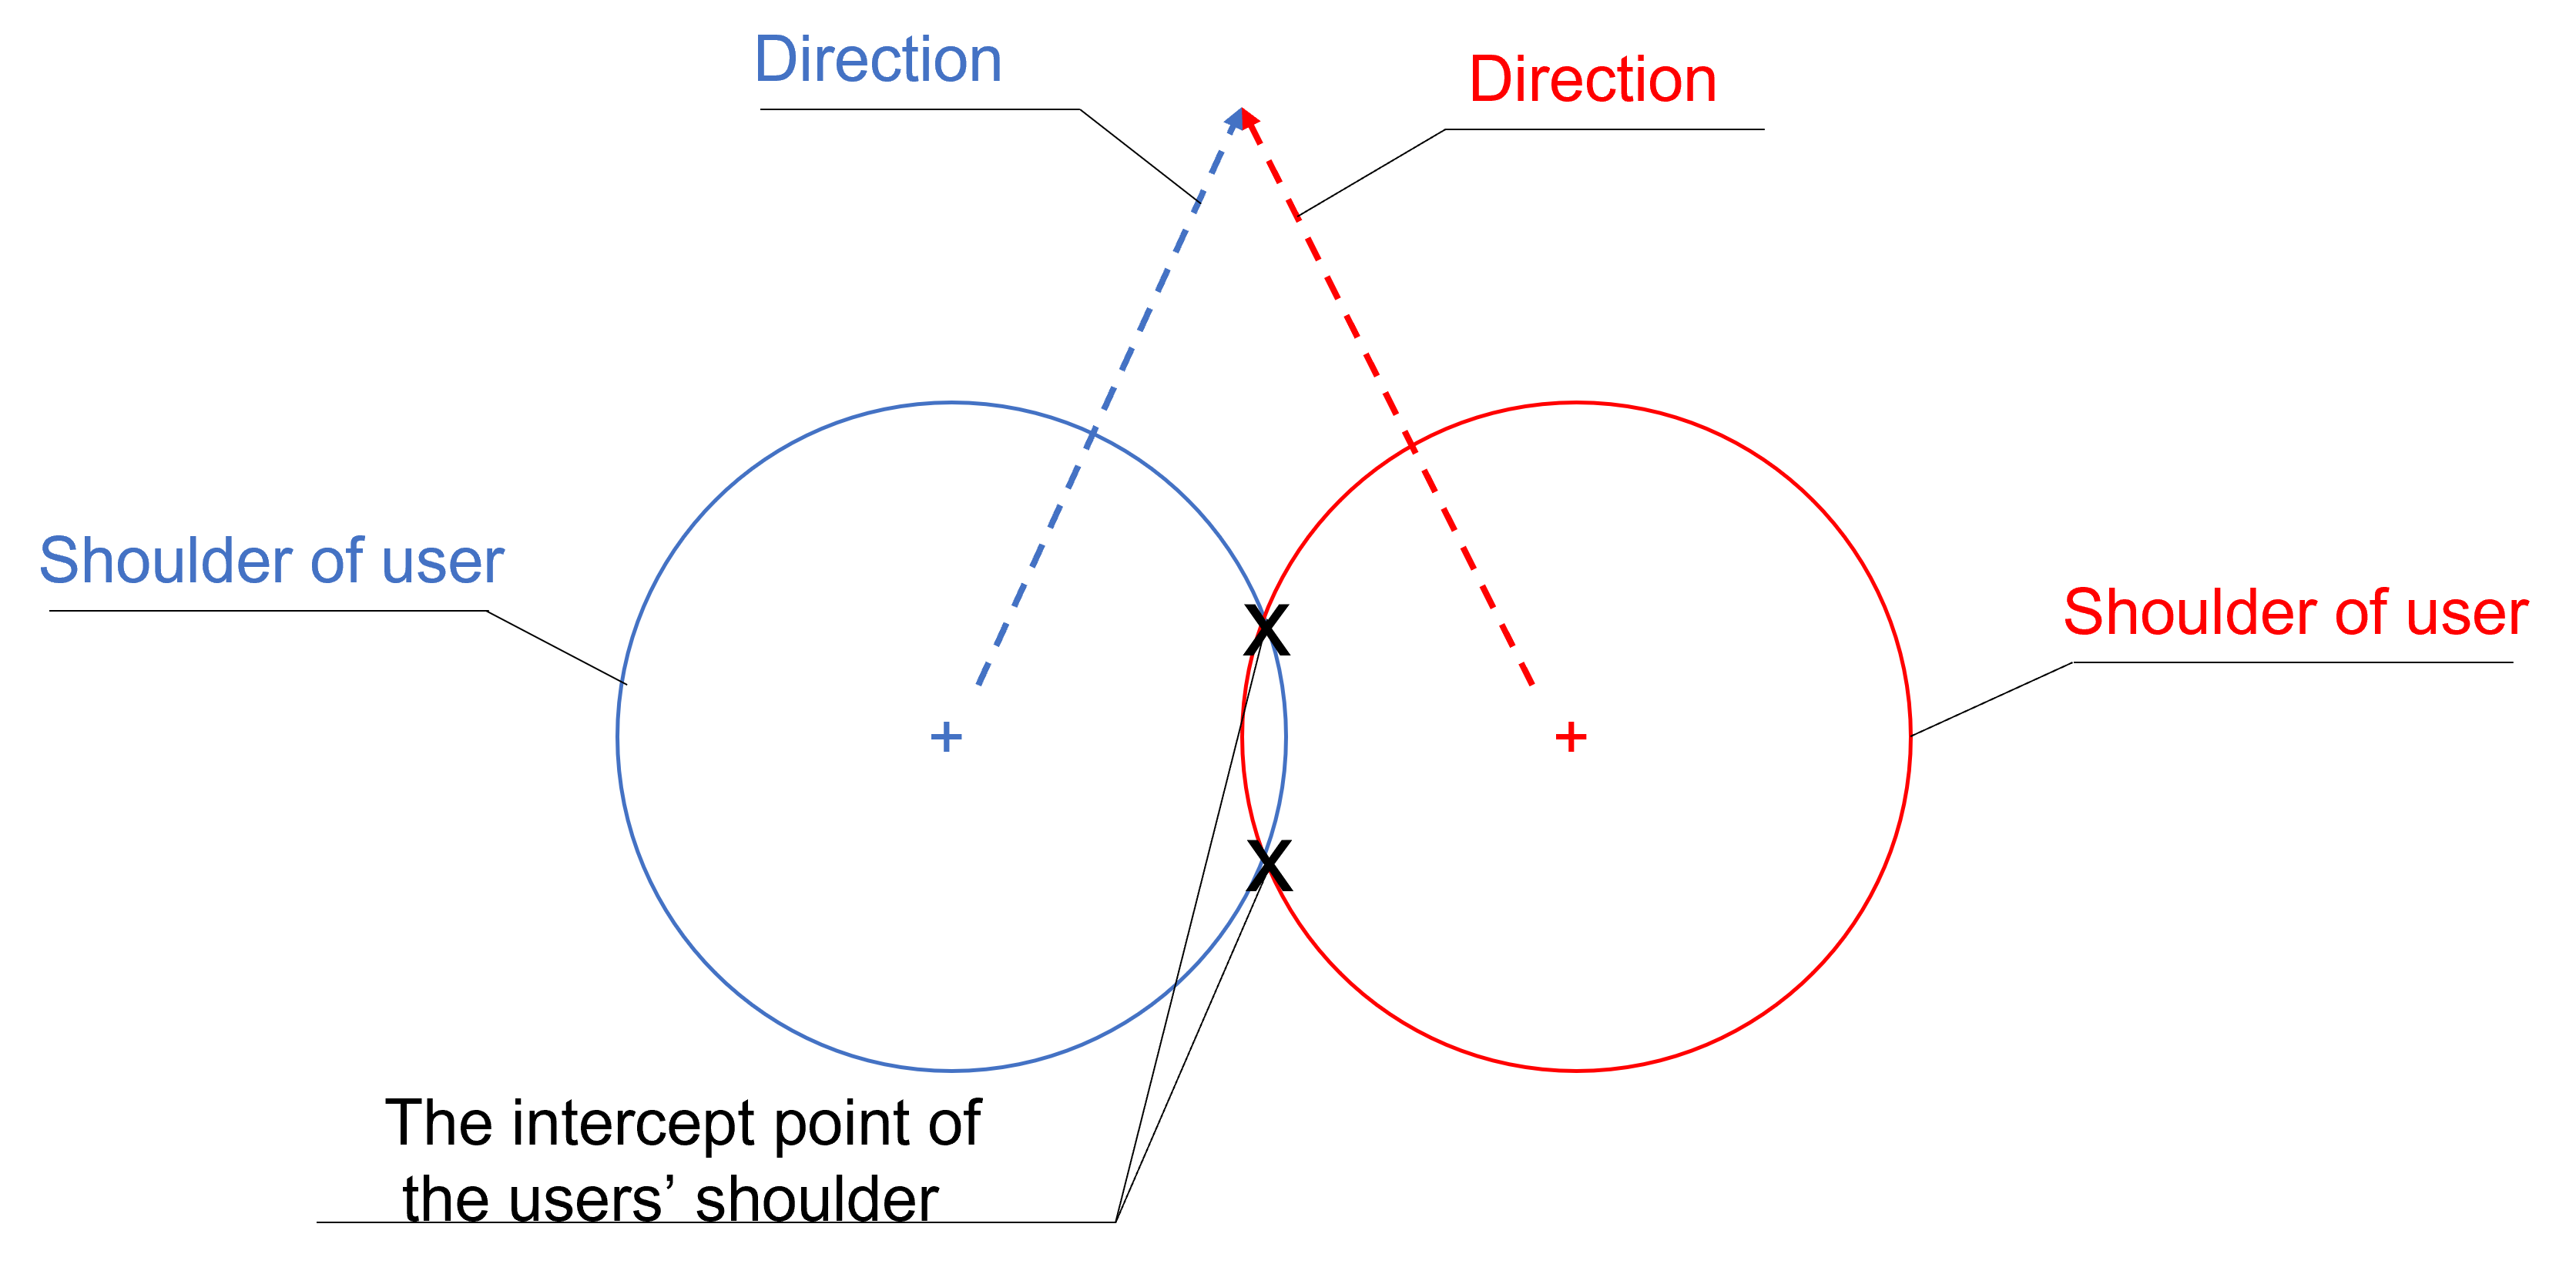
\includegraphics[width=1.0\textwidth]{Pictures/Collision detection_edited.png}%imagine location
	\caption{Collision detection.}\label{fig:Collision detection}%use name for ref.
\end{figure}

%Collision detection formula:

%\[
%(x - h)^2+(y-k)^2  = r^2
% \]
%\[
%(x - h_1)^2+(y - k_1)^2  = (x - h_2)^2+(y - k_2)^2
% \]
%\\

%\hspace{10mm} x  = The values in the horizontal axis on the circle formula.

%\hspace{10mm} y = The values in the vertical axis on the circle formula.

%\hspace{10mm} r = Radius of circle

%\hspace{10mm} h = Position of user in the horizontal axis.

%\hspace{10mm} k = Position of user in the vertical axis.
%\\
\newpage

\subsubsection{Collision avoidance}
The method takes a strategy where a collision avoidance for two users is applied to every two users who will collide with each other, repeatedly for multiple users. When a collision is predicted, the method marks two offset points on an imaginary line that is perpendicular to the facing direction of each user and calculates the distance between all the diagonal pairs of the offset points to find the longest distance. The two users are steered to their own offset point with the longest distance to avoid a collision by applying translation gains and time-dependent rotational gains. The rotation direction of steering is prescribed by the offset point. The process is shown in Fig.~\ref{fig:S2OC_detect}-\ref{fig:S2OC_Steer2Offset}.
\begin{figure}[H]\centering
	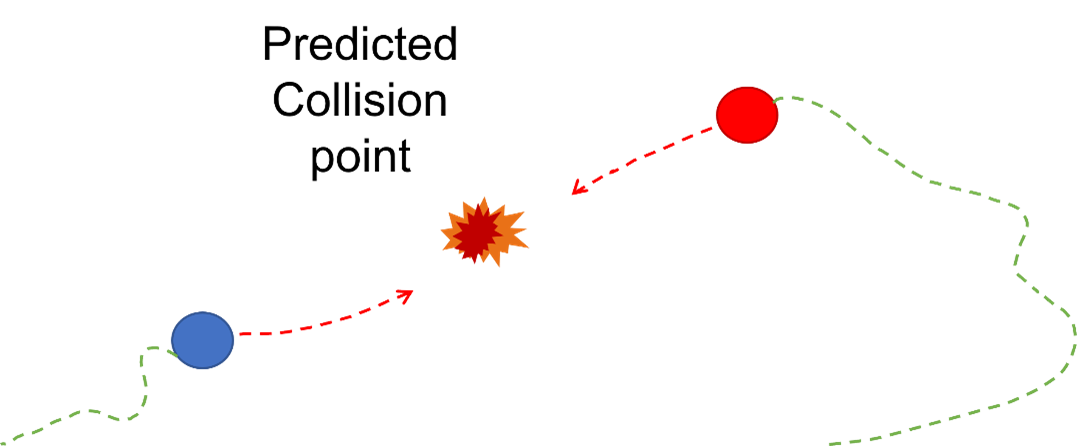
\includegraphics[width=0.8\textwidth]{Pictures/Predict the collision with the other user.png}%imagine location
	\caption{Predict a collision with two users.}\label{fig:S2OC_detect}%use name for ref.
\end{figure}
\begin{figure}[H]\centering
	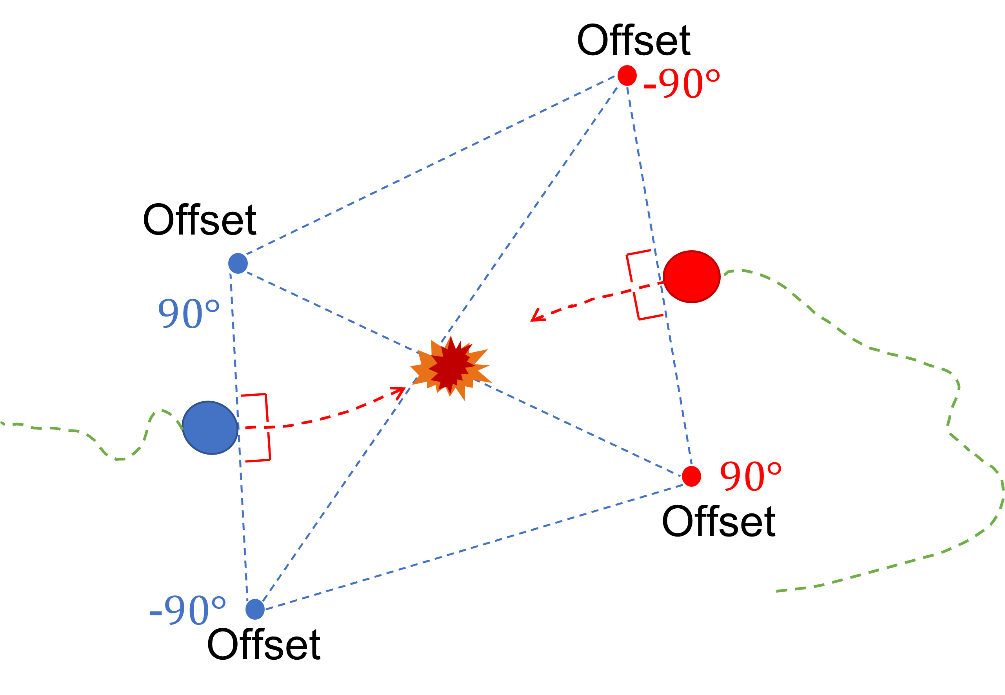
\includegraphics[width=0.8\textwidth]{Pictures/Mark offset points on the imaginary line which is perpendicular to the facing direction of each user.png}%imagine location
	\caption{Mark offset points on an imaginary line which is perpendicular to the facing direction of each user.}\label{fig:S2OC_mark}%use name for ref.
\end{figure}

\begin{figure}[H]\centering
	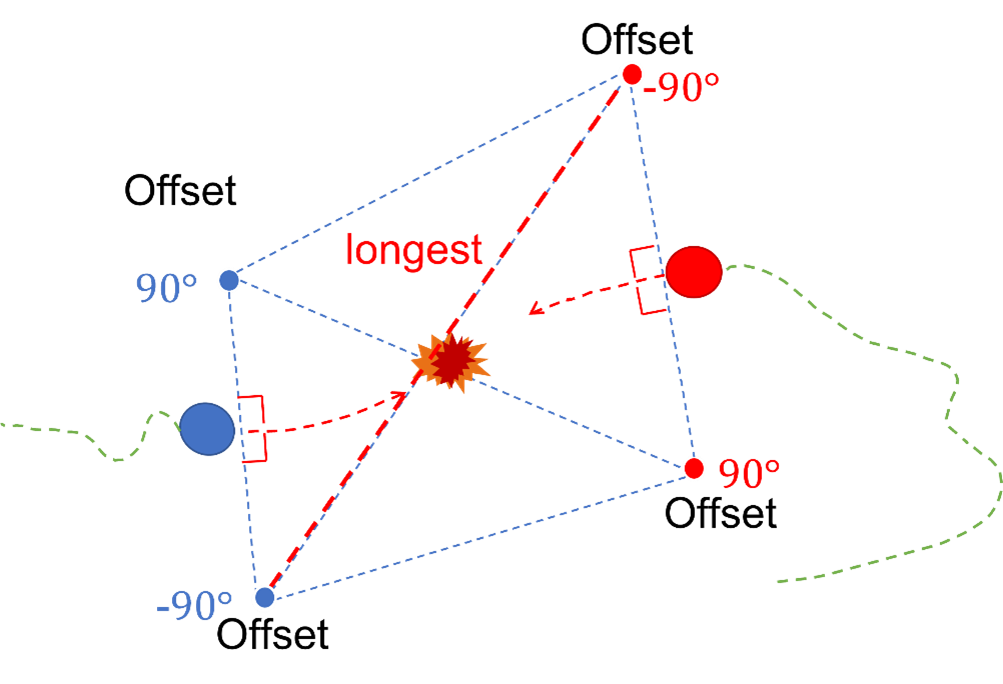
\includegraphics[width=0.8\textwidth]{Pictures/Find the longest distance.png}%imagine location
	\caption{Find the longest distance between all the diagonal pairs of offset points.}\label{fig:S2OC_FindLongDis}%use name for ref.
\end{figure}
\begin{figure}[H]\centering
	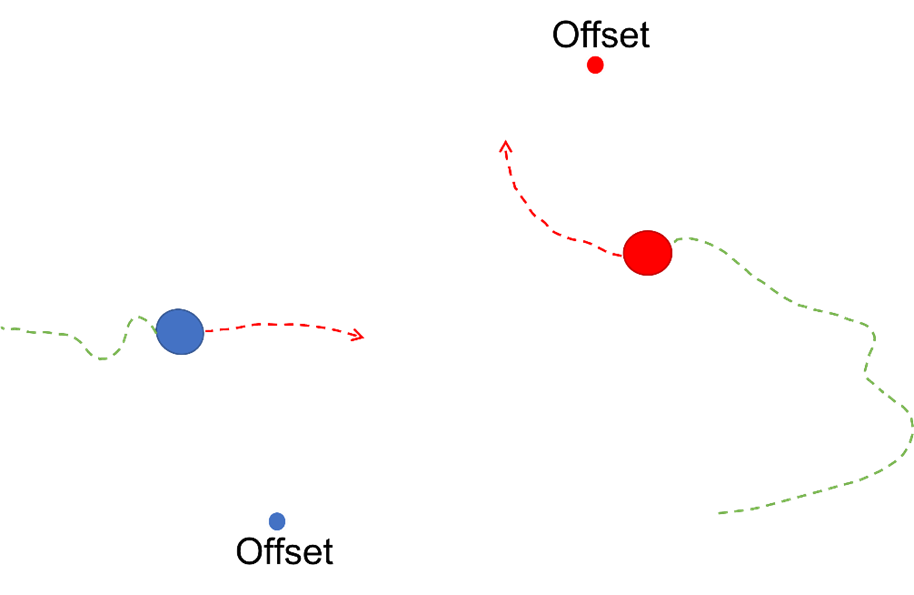
\includegraphics[width=0.8\textwidth]{Pictures/Steer each user to offset point.png}%imagine location
	\caption{Steer each user to his/her offset point.}\label{fig:S2OC_Steer2Offset}%use name for ref.
\end{figure}


\newpage
\section{Motion sickness}
When your brain receives conflicting signals about movement, your brain responses to it as motion sickness. In the context of VR, this effectively means that if you stay stationary while a virtual environment around you moves, equilibrium of your brain is disrupted, and you become nauseated~\cite{5298757}.



There are various factors to consider when it comes to why motion sickness happens in VR and what affects it. T. van Gemert et al.~\cite{9419312} discuss the most important factors and measurements of VR motion sickness. Duration and optical flow in a virtual environment are important factors of motion sickness in terms of software. For hardware factors such as refresh rate of HMDs, display flicker, input lag, and range of view all are linked to an increase in the prevalence of VR sickness. P. Bimberg et al.~\cite{9090573} used Simulator Sickness Questionnaire (SSQ) to measure simulator sickness scores. A simulator sickness score is computed by symptoms such as nausea, blurred vision, headache etc.
A. Singla et al.~\cite{7965658} compared the quality of different VR contents for two HMDs (HTC Vive and Oculus Rift) by SSQ. The results indicate that HTC Vive offers slightly greater integral quality than Oculus Rift. Contents and resolution have a significant impact to simulator sickness~\cite{o2021preventing}. For motion sickness, the symptom scores can reduce by 40\% after using  VR training for motion sickness.

In this thesis, to evaluate motion sickness, subjects are asked to reply to SSQ to check for their abnormal symptoms.
%To evaluate motion sickness, this thesis applied a symptom questionnaire is therefore conducted after being tested to explore the resulting abnormalities and to ensure the user's safety\cite{Norman2018EvaluationOV}.


 
 